\documentclass{standalone}

\begin{document}

\section{Übung 3}

\subsection{DISCLAIMER - BITTE LESEN}
Hinterfragt (wie ihr es immer tun solltet) unsere Lösungen auf alle Fälle und versucht sie nachzuvollziehen. 
Wir können Fehler nicht ausschließen. Meldet euch gerne, wenn euch etwas aufgefallen ist, bevor einige Helden doch wieder nur die Lösungen auswendig lernen! (wobei Durchfallen dann verdient wäre\dots)
Korrekturen werden wir nachträglich noch einpflegen und (bald) auch immer den aktuellen Stand des Dokuments zur Verfügung stellen\dots aber eins nach dem anderen.
\\ \\
Beste Grüße \\
\textit{Euer Autoren-Team}

\subsection{Aufgabe 3.1}

$$
    v_1 = \begin{pmatrix} 1 \\ 0 \end{pmatrix},
    v_2 = \begin{pmatrix} 2 \\ 1 \end{pmatrix},
    v_3 = \begin{pmatrix} 5 \\ 3 \end{pmatrix},
    v_4 = \begin{pmatrix} 0 \\ 4 \end{pmatrix},
    v_5 = \begin{pmatrix} 2 \\2  \end{pmatrix}
$$

\begin{enumerate}[a)]
    \item $ \langle v_1,v_2 \rangle = \begin{pmatrix}
        1 \\ 0 
    \end{pmatrix}x
    \cdot \begin{pmatrix}
        2 \\ 1
    \end{pmatrix}
    = 1 \cdot 2 + 0 \cdot 1 = 2$
    \item $ \langle v_2,v_3 \rangle = \begin{pmatrix}
        2 \\ 1
    \end{pmatrix}
    \cdot \begin{pmatrix}
        5 \\ 3
    \end{pmatrix}
    = 2 \cdot 5 + 1 \cdot 3 = 13$
    % -- c) --
    \item $ \langle v_3,v_4 \rangle = \begin{pmatrix}
        5 \\ 3
    \end{pmatrix}
    \cdot \begin{pmatrix}
        0 \\ 4
    \end{pmatrix}
    = 5 \cdot 0 + 3 \cdot 4 = 12$
    \item $ \langle v_1,v_4 \rangle = \begin{pmatrix}
        1 \\ 0
    \end{pmatrix}
    \cdot \begin{pmatrix}
        0 \\ 4
    \end{pmatrix}
    = 1 \cdot 0 + 0 \cdot 4 = 0 $
    % -- d) --
    
   
    

\end{enumerate}

\subsection{Aufgabe 3.2}

$$
    v_1 = \begin{pmatrix} 1 \\ 0 \\ 1 \end{pmatrix},
    v_2 = \begin{pmatrix} 2 \\ 1 \\ 3 \end{pmatrix},
    v_3 = \begin{pmatrix} 5 \\ 3 \\ -2 \end{pmatrix},
    v_4 = \begin{pmatrix} 0 \\ 4 \\ 6 \end{pmatrix}
$$

\begin{enumerate}[a)]
    \item Skalarprodukte und Kreuzprodukte
    \begin{enumerate}
        % ---- (i)
        \item $\langle v_1,v_2 \rangle = 
        \begin{pmatrix}
            1 \\ 0 \\ 1
        \end{pmatrix}
        \cdot \begin{pmatrix}
            2 \\ 1 \\ 3
        \end{pmatrix}
        = 1 \cdot 2 + 0 \cdot 1 + 1 \cdot 3 = 5$ \\
        
        $ v_1 \times v_2 = 
        \begin{pmatrix}
            1 \\ 0 \\ 1
        \end{pmatrix}
        \times \begin{pmatrix}
            2 \\ 1 \\ 3
        \end{pmatrix}
        = \begin{pmatrix}
            0 \cdot 3 - 1 \cdot 1 \\ 1 \cdot 2 - 1 \cdot 3 \\ 1 \cdot 1 - 0 \cdot 2
        \end{pmatrix}
        = \begin{pmatrix}
            -1 \\ -1 \\ 1
        \end{pmatrix}$

        % ---- TRENNUNG (ii)
        \item $\langle v_2,v_3 \rangle = 
        \begin{pmatrix}
            2 \\ 1 \\ 3
        \end{pmatrix}
        \cdot \begin{pmatrix}
            5 \\ 3 \\ -2
        \end{pmatrix}
        = 2 \cdot 5 + 1 \cdot 3 + 3 \cdot (-2) = 7$ \\
        
        $ v_2 \times v_3 = 
        \begin{pmatrix}
            2 \\ 1 \\ 3
        \end{pmatrix}
        \times \begin{pmatrix}
            5 \\ 3 \\ -2
        \end{pmatrix}
        = \begin{pmatrix}
            1 \cdot (-2) - 3 \cdot 3 \\ 3 \cdot 5 - 2 \cdot (-2) \\ 2 \cdot 3 - 1 \cdot 5
        \end{pmatrix}
        = \begin{pmatrix}
            -11 \\ 19 \\ 1
        \end{pmatrix}$

        % ---- TRENNUNG(iii)
        \item $\langle v_3,v_4 \rangle = 
        \begin{pmatrix}
            5 \\ 3 \\ -2
        \end{pmatrix}
        \cdot \begin{pmatrix}
            0 \\ 4 \\ 6
        \end{pmatrix}
        = 5 \cdot 0 + 3 \cdot 4 + (-2) \cdot 6 = 0$ \\
        
        $ v_3 \times v_4 = 
        \begin{pmatrix}
            5 \\ 3 \\ -2
        \end{pmatrix}
        \times \begin{pmatrix}
            2 \\ 1 \\ 3
        \end{pmatrix}
        = \begin{pmatrix}
            3 \cdot 6 - (-2) \cdot 4 \\ (-2) \cdot 0 - 5 \cdot 6 \\ 5 \cdot 4 - 3 \cdot 0
        \end{pmatrix}
        = \begin{pmatrix}
            26 \\ -30 \\ 20
        \end{pmatrix}$
    \end{enumerate}
    \item Senkrecht
    \begin{enumerate}
        \item $\langle v_1,v_2 \rangle = 5$, nicht senkrecht
        \item $\langle v_1,v_3 \rangle = 3$, nicht senkrecht
        \item $\langle v_1,v_4 \rangle = 6$, nicht senkrecht
        \item $\langle v_2,v_3 \rangle = 7$, nicht senkrecht
        \item $\langle v_2,v_4 \rangle = 22$, nicht senkrecht
        \item $\langle v_3,v_4 \rangle = 0$, senkrecht
    \end{enumerate}
    \item Normen
    \begin{enumerate}
        \item $\norm{v_1} = \sqrt{1^2 + 0^2 + 1^2} = \sqrt{2} \\ v_{1,n} = \frac{1}{\sqrt{2}}\begin{pmatrix} 1 \\ 0 \\ 1 \end{pmatrix}$
        \item $\norm{v_2} = \sqrt{2^2 + 1^2 + 3^2} = \sqrt{14} \\ v_{2,n} = \frac{1}{\sqrt{14}}\begin{pmatrix} 2 \\ 1 \\ 3 \end{pmatrix}$
        \item $\norm{v_3} = \sqrt{5^2 + 3^2 + (-2)^2} = \sqrt{38} \\ v_{3,n} = \frac{1}{\sqrt{38}}\begin{pmatrix} 5 \\ 3 \\ -2 \end{pmatrix}$
        \item $\norm{v_4} = \sqrt{0^2 + 4^2 + 6^2} = \sqrt{52} \\ v_{4,n} = \frac{1}{\sqrt{52}}\begin{pmatrix} 0 \\ 4 \\ 6 \end{pmatrix}$
    \end{enumerate}
    \item Winkel - die Werte der Skalarprodukte und Normen können aus a) und c) übernommen werden
    \begin{enumerate}
        \item $\cos \angle (v_1,v_2) = \frac{\langle v_1,v_2 \rangle}{\norm{v_1} \norm{v_2}} = 
        \frac{5}{\sqrt{2}\sqrt{14}} = \frac{5}{\sqrt{28}}$
        \item $\cos \angle (v_2,v_3) = \frac{\langle v_2,v_3 \rangle}{\norm{v_2} \norm{v_3}} = 
        \frac{7}{\sqrt{14}\sqrt{38}} = \frac{5}{\sqrt{546}}$
        \item $\cos \angle (v_3,v_4) = \frac{\langle v_3,v_4 \rangle}{\norm{v_3} \norm{v_4}} = 
        \frac{0}{\sqrt{38}\sqrt{52}} = 0$
    \end{enumerate}
    \item Berechnen
    \begin{enumerate}
        \item $\langle v_1,6v_2 + 7v_4 \rangle = 
        \begin{pmatrix}
            1 \\ 0 \\ 1
        \end{pmatrix}
        \cdot \left(\begin{pmatrix}
            12 \\ 6 \\ 18
        \end{pmatrix}
        + \begin{pmatrix}
            0 \\ 28 \\ 42
        \end{pmatrix}\right)
        = \begin{pmatrix}
            1 \\ 0 \\ 1
        \end{pmatrix}
        \cdot \begin{pmatrix}
            12 \\ 34 \\ 60
        \end{pmatrix}
        = 1 \cdot 12 + 1 \cdot 60 = 72$
        \item $6\langle v_1, v_2 \rangle + 7\langle v_1,v_4 \rangle = 6\cdot 5 + 7\cdot (1\cdot 0+0\cdot 4 + 1 \cdot 6) = 30 + 42 = 72$
    \end{enumerate}
\end{enumerate}

\subsection{Aufgabe 3.4}
Abstand der Punkte entspricht der Norm des Vektors zwischen den zwei Punkten
\begin{enumerate}[a)]
    \item $ a = (2,1)^T, b = (-3,1)^T \\
    d = \norm{\overrightarrow{ab}} = \norm{\begin{pmatrix}
        2 \\ 1
    \end{pmatrix}
    -\begin{pmatrix}
        -3 \\ 1
    \end{pmatrix}}
    = \norm{\begin{pmatrix}
        5 \\ 0
    \end{pmatrix}} = 5$

    \item $ a = (1,0,0)^T, b = (0,1,0)^T \\
    d = \norm{\overrightarrow{ab}} = \norm{\begin{pmatrix}
        1 \\ 0 \\ 0
    \end{pmatrix}
    -\begin{pmatrix}
        0 \\ 1 \\ 0
    \end{pmatrix}}
    = \norm{\begin{pmatrix}
        1 \\ -1 \\ 0
    \end{pmatrix}} = \sqrt{2}$

    \item $ a = (5,4,3)^T, b = (-5,-4,-3)^T \\
    d = \norm{\overrightarrow{ab}} = \norm{\begin{pmatrix}
        5 \\ 4 \\ 3
    \end{pmatrix}
    -\begin{pmatrix}
        -5 \\ -4 \\ -3
    \end{pmatrix}}
    = \norm{\begin{pmatrix}
        10 \\ 8 \\ 6
    \end{pmatrix}} = \sqrt{200}$
\end{enumerate}

\subsection{Aufgabe 3.5}
Koordinatenachsen (2-D-Vektor, also x- und y-Achse):
$$ v_1 = (1,0)^T,\, \norm{v_1} = 1 \; ; v_2 = (0,1)^T,\,\norm{v_2} = 1$$
$$a = (2,5)^T, \, \norm{a} = \sqrt{29}$$

Die Zwischenrechnung für Skalarprodukte und Normen überspringe ich an dieser Stelle, da genügend Beispiele in den vorherigen Aufgaben liegen.
\begin{enumerate}[a)]
    \item x-Achse: $\angle(a, v_1) = \arccos \frac{\langle a,v_1\rangle}{\norm{a}\norm{v_1}}
    = \arccos \frac{2}{\sqrt{29}}$
    \item x-Achse: $\angle(a, v_2) = \arccos \frac{\langle a,v_2\rangle}{\norm{a}\norm{v_2}}
    = \arccos \frac{5}{\sqrt{29}}$
\end{enumerate}

\subsection{Aufgabe 3.6}
\begin{enumerate}[a)]
    \item $$a=(a_1,a_2)^T \, ; w = (w_1, w_2)^T $$
    Senkrecht bedeutet, dass das Skalarprodukt der Vektoren $= 0$ sein muss. Es gilt also folgende Gleichung zu lösen:
    $$a_1 \cdot w_1 + a_2 \cdot w_2 = 0$$
    Dabei sind $a_1$ und $a_2$ bekannt. Da die Gleichung zwei Unbekannte hat, gibt es (im allgemeinen Fall) unendlich viele Lösungen, außer einer der Summanden ist $= 0$.
    Dasselbe gilt für $\mathbb{R}^3$, außer dass die Lösung dann eindeutig ist, wenn zwei der Summanden $= 0$ sind.
    Man kann also, bis auf einen, beliebige Werte für $w_i$ annehmen und den letzen auflösen.\\

    ERGÄNZUNG: Durch die Vorgabe, dass der Vektor die Länge 1 haben soll, haben wir eine zusätzliche Gleichung/Nebenbedingung mit
    $$\sum_{k=1}^{n}w_i^2=1$$
    Dabei entspricht $n$ der Anzahl der Dimensionen des Vektors. Diese Bedingung kann so erfüllt werden, dass zwar immer noch alle bis auf ein $w_i$ frei gewählt werden, der Vektor am Ende nur zusätzlich normiert wird. Somit muss die Gleichung nicht im Gleichungssystem berücksichtigt werden.
    
    \begin{align}
        -3 w_1 + 0 w_2 &= 0 \\
        -3w_1 &= 0 \\
        w_1 &=0
    \end{align}
    $w_2$ ist hier beliebig wählbar. Da die Länge des Vektors $=1$ sein soll, ist $w_2 = 1$. Somit ist $\norm{w} = 1$.

    \item $$ b = (0,0,0)^T\, ; w = (w_1,w_2,w_3)^T $$
    \begin{align}
        0w_1 + 0w_2 + 0w_3 &= 0 \\
        0 + 0 + 0 = 0
    \end{align}
    $w_1$, $w_2$ und $w_3$ sind beliebig wählbar unter der Nebenbedigung
    $$w_1^2 +w_2^2+w_3^2=1$$, damit der Vektor die Länge 1 hat.

    \item $$ c = (1,1,1)^T \, ; w = (w_1,w_2,w_3)^T $$
    Da wir eine Gleichung und drei Unbekannte haben, wählen wir einfach $w_1$ und $w_2 = 1$ 
    \begin{align}
        1w_1 + 1w_2 + 1w_3 &= 0 \\
        1 + 1 + w_3 &= 0 \\
        w_3 &= -2
    \end{align}
    Damit ist $w = (1,1,-2)^T$ und muss nun noch normiert werden. Mit $\norm{w} = \sqrt{6}$ ergibt sich 
    $$ w_n = \frac{1}{\sqrt{6}}\begin{pmatrix}
        1 \\ 1 \\ -2
    \end{pmatrix}$$

    \item $$ d = (-5,k,0)^T, \, k \in \mathbb{R} \; ; w = (w_1,w_2,w_3)^T $$
    Da wir eine Gleichung und drei Unbekannte haben, wählen wir einfach $w_2$ und $w_3 = 1$. $w_1$ oder $w_2$ sollten dabei berechnet werden, da $w_3$ durch die Multiplikation mit 0 sowieso wegfällt und sonst ein Spezialfall herrscht. 
    \begin{align}
        -5w_1 + kw_2 + 0w_3 &= 0 \\
        -5w_1 + k &= 0 \\
        w_1 = \frac{1}{5}k
    \end{align}
    Damit ist $w = (\frac{1}{5}k,1,1)$ und muss noch normiert werden. Mit $\norm{w} = \sqrt{\frac{1}{25}k + 2}$ ergibt sich
    $$ w_n = \frac{1}{\sqrt{\frac{1}{25}k + 2}}$$
\end{enumerate}

\subsection{Aufgabe 3.7}
\begin{enumerate}[a)]
    \item $$a = (2,1)^T\; ; b = (3,2)^T$$
    \begin{align}
        a_{\parallel} &= \frac{\langle a,b\rangle}{\norm{b}}b \\
        a_{\bot} &= a - a_{\parallel}
    \end{align}
    Damit 
    \begin{align}
        \norm{b} &= \sqrt{13} \\
        a_{\parallel} &= \frac{8}{\sqrt{13}}(3,2)^T \\
        a_{\bot} &= (2,1)^T - \frac{8}{\sqrt{13}}(3,2)^T
    \end{align}

    \item $$a = (2,6)^T\; ; b = (-9,3)^T$$
    \begin{align}
        \norm{b} &= \sqrt{90} \\
        a_{\parallel} &= \frac{0}{\sqrt{90}}(-9,3)^T = 0\\
        a_{\bot} &= (2,6)^T - (0,0)^T = (2,6)^T 
    \end{align}

    \item $$c = (4,-1,7)^T\; ; d = (2,3,-6)^T$$
    \begin{align}
        \norm{d} &= 7 \\
        c_{\parallel} &= -\frac{37}{7}(2,3,-6)^T \\
        c_{\bot} &= (4,-1,7)^T + \frac{37}{7}(2,3,-6)^T
    \end{align}

    \item $$c = (1,0,0)^T\; ; d = (0,1,1)^T$$
    \begin{align}
        \norm{d} &= \sqrt{2} \\
        c_{\parallel} &= \frac{0}{\sqrt{2}}(0,1,1)^T = 0 \\
        c_{\bot} &= (1,0,0)^T - (0,0,0)^T = (1,0,0)^T
    \end{align}
\end{enumerate}

\subsection{Aufgabe 3.8}
Die Kantenlänge und Ausrichtung des Dreiecks im $\mathbb{R}^3$ ist nicht vorgegeben, zudem ist nur die Rede von einem einzigen Dreieck.
Das heißt, dass wir einfach ein beliebiges definieren können.
Das Dreieck wird anhand von drei Punkten definiert.
Ein gleichseitiges Dreieck hat drei Seiten mit derselben Kantenlänge.
Daraus ergibt sich unmittelbar, dass die inneren Winkel des Dreiecks identisch, und damit jeweils $60\circ$, bzw $\frac{\pi}{3}$ betragen.

Der erste Ankerpunkt liegt in auf $a_1 = (0,0)^T$, weil es am einfachsten ist. Die Kantenlänge legen wir auf 1 fest.
Die erste Kante können wir beliebig legen (Hauptsache Länge $= 1$). Dann wählen wir einfach $a_2 = (1,0)^T$.

Den dritten Punkt erhalten wir über einfach Trigonometrie. Wenn wir einen Einheitskreis um $(0,0)^T$ herum legen, brauchen wir den Punkt auf $60\circ$ im Kreis.
Diesen erhalten wir durch

$$a_3 = \begin{pmatrix}
    \cos \frac{\pi}{3} \\
    \sin \frac{\pi}{3}
\end{pmatrix}
= \begin{pmatrix}
    \frac{1}{2} \\
    \frac{\sqrt{3}}{2}
\end{pmatrix}$$

Damit ist das Dreieck
$$ a_1 = (0,0)^T \; ; a_2 = (1,0)^T \; ; a_3 = (\frac{1}{2}, \frac{\sqrt{3}}{2})$$

Über einen Faktor $k$ oder einer Transformationsmatrix mit $$\begin{pmatrix}
    \cos \phi & -\sin \phi & x\\
    \sin \phi & \cos \phi & y
\end{pmatrix}$$
kann dieses Dreieck beliebig um den Winkel $\phi$ verdreht, den Vektor $(x,y)^T$ verschoben, oder seine Kantenlänge um $k$ skaliert werden.

\subsection{Aufgabe 3.9}
\begin{itemize}
    \item Gleichseitig: alle Seiten sind gleich lang
    \item Gleichschenklig: zwei Seiten sind gleich lang (ergibt sich aus zwei gleich großen Winkeln)
    \item Rechtwinklig: ein rechter Winkel vorhanden
\end{itemize}
Ansatz: Für alle Dreiecke die Vektoren der Kanten, ihre Beträge und Skalarprodukte bestimmen.

PS: Schon klar, dass man das meiste direkt aus den Punkten heraus erkennen kann, aber dennoch der Vollständigkeit halber die Rechnung dazu.

\begin{enumerate}[a)]
    \item $$ a = (0,4)^T \; ; b = (-4,0)^T \; c = (0,0)^T$$
    \begin{align}
        \overrightarrow{ab} &= (-4,-4)^T \\
        \overrightarrow{bc} &= (4, 0)^T \\
        \overrightarrow{ca} &= (0,4) \\
        \norm{\overrightarrow{ab}} &= \sqrt{32} \\
        \norm{\overrightarrow{bc}} &= 4 \\
        \norm{\overrightarrow{ca}} &= 4 \\
        \langle \overrightarrow{ab}, \overrightarrow{bc} \rangle &= -16 \\
        \langle \overrightarrow{bc}, \overrightarrow{ca} \rangle &= 0 \\
        \langle \overrightarrow{ca}, \overrightarrow{ab} \rangle &= -16 \\
    \end{align}
    Rechtwinklig und gleichschenklig.

    \item $$ a = (2,3)^T \; ; b = (-3,2)^T \; c = (1,4)^T$$
    \begin{align}
        \overrightarrow{ab} &= (-5,-1)^T \\
        \overrightarrow{bc} &= (4, 2)^T \\
        \overrightarrow{ca} &= (1,-1) \\
        \norm{\overrightarrow{ab}} &= \sqrt{26} \\
        \norm{\overrightarrow{bc}} &= \sqrt{20} \\
        \norm{\overrightarrow{ca}} &= \sqrt{2} \\
        \langle \overrightarrow{ab}, \overrightarrow{bc} \rangle &= -22 \\
        \langle \overrightarrow{bc}, \overrightarrow{ca} \rangle &= 2 \\
        \langle \overrightarrow{ca}, \overrightarrow{ab} \rangle &= -4 \\
    \end{align}
    Nichts.

    \item $$ a = (0,1)^T \; ; b = (-1,0)^T \; c = (0,-1)^T$$
    \begin{align}
        \overrightarrow{ab} &= (-1,-1)^T \\
        \overrightarrow{bc} &= (1, -1)^T \\
        \overrightarrow{ca} &= (0,2) \\
        \norm{\overrightarrow{ab}} &= \sqrt{2} \\
        \norm{\overrightarrow{bc}} &= \sqrt{2} \\
        \norm{\overrightarrow{ca}} &= 2 \\
        \langle \overrightarrow{ab}, \overrightarrow{bc} \rangle &= 0 \\
        \langle \overrightarrow{bc}, \overrightarrow{ca} \rangle &= -2 \\
        \langle \overrightarrow{ca}, \overrightarrow{ab} \rangle &= -2 \\
    \end{align}
    Gleichschenklig und rechtwinklig.
\end{enumerate}

% --- OZZIS TEIL ---

\subsection{Aufgabe 3.10}
\begin{enumerate}[a)]
    \begin{figure}[htbp]
        \centering
        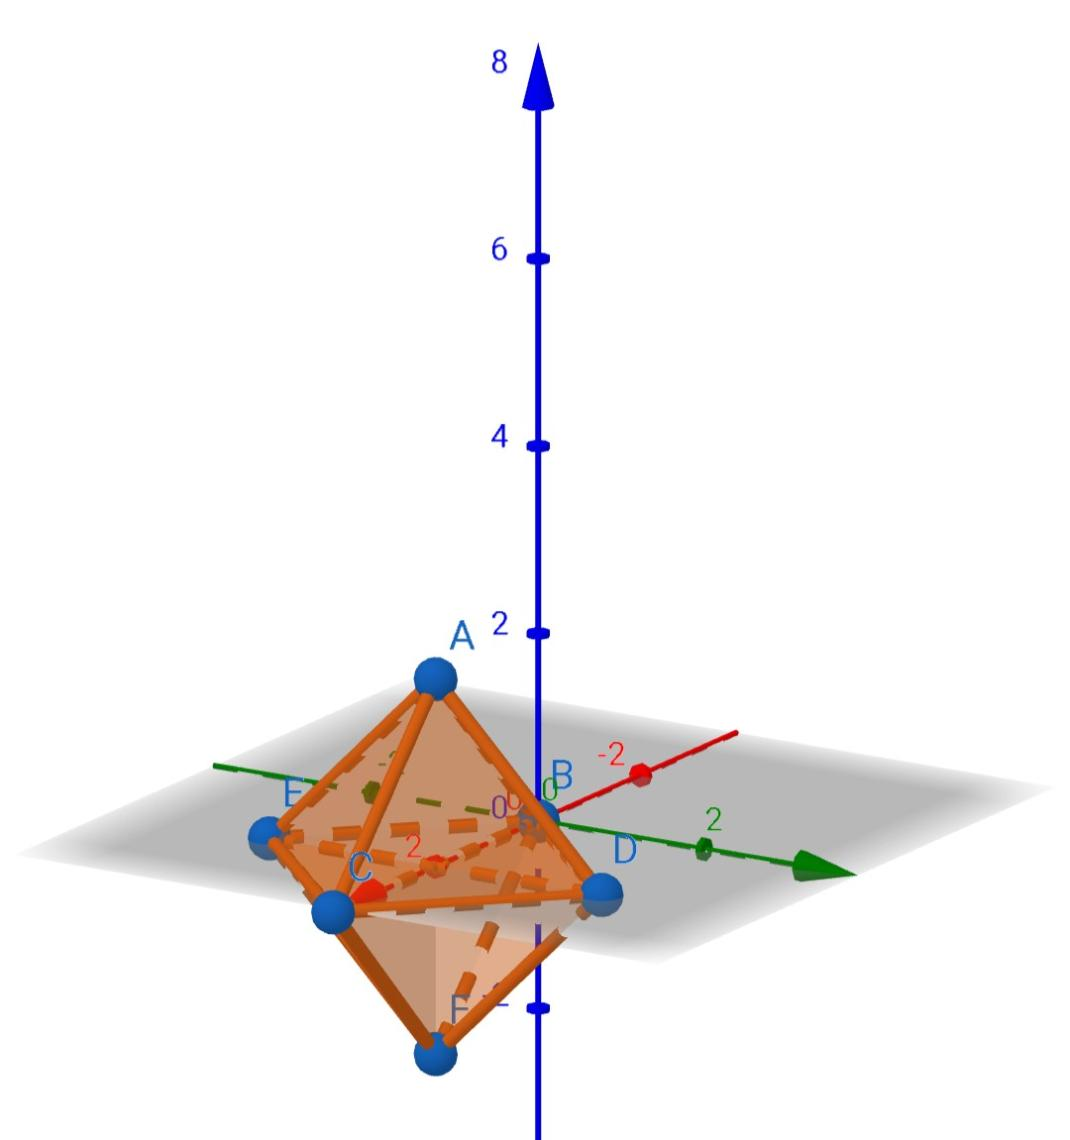
\includegraphics[width=6cm]{img/3_10_a}
        \caption{Dieses Objekt heisst Octahedron.}
    \end{figure}
    \FloatBarrier
    \item $\parallel  \overline{ab}  \parallel =$ 4. Die sind einfach auf der gleichen Gerade. 
    \item Man kann diese Objekts Volume durch zwei Methoden berechnen. Eins, kann man ein Orthagon zu dem Ebene EBDC machen dann das Volume für ein Pyramid rechen und dann mit 2 multiplizieren. Zweite method ist einfacher. Da die Seitenlaenge (a=2.83) gleich sind, dies Objekt ist ein Regulaeres Octahedron, mit $\frac{a^3}{3 \sqrt{2}}$ rechen. Also die Antwort lautet: $\simeq$10.68
\end{enumerate}

\subsection{Aufgabe 3.11}
\begin{enumerate}[a)]
    \item[a)] 90 $\circ$  gedrehtem $\vec{b}$ ist   $\vec{b}^{T}(2,1)$. Durch das Cosinusverfahren $cos( \alpha)= \frac{\langle a,b \rangle}{  \parallel a  \parallel  .   \parallel b \parallel  \ }$   bestimmt man der Winkel. Also die Antwort lautet: $arccos(\frac{3}{\sqrt{10}}) \simeq 18 \circ$ 
    \item[b)] Gleichermassen von der obere Teilaufgabe, benutz man das Cosinusverfahren. Aber $\vec{b}^{T}$ lautet hier $\vec{b}^{T}(-1,2)$. Also die Antwort lautet: $arccos(\frac{1}{\sqrt{10}}) \simeq 71 \circ$ 
\end{enumerate}

\subsection{Aufgabe 3.12}
\begin{enumerate}[a)]
    \item[a)]$\vec{a}= (X_1,Y_1)$ und $\vec{b}=(X_2,Y_2)$ dann ist $\vec{c}= \vec{a}+\vec{b}$ dem Seitenmitten von $\vec{a}$ und $\vec{b}$ ist $\frac{1}{2}( \vec{a})  \frac{1}{2}( \vec{b})$. Die Seitenlaenge von $\vec{c}$ ist  $ \sqrt{ (X_1-X_2)^2 + (Y_1-Y_2)^2} $. Die Seitenlaenge von die Seitenmittenvektor ist   $\sqrt{ (\frac{1}{2}X_1-\frac{1}{2}X_2)^2 + (\frac{1}{2}Y_1-\frac{1}{2}Y_2)^2}$. Durch ausklammern sieht man, dass es $\frac{1}{2}\sqrt{ (X_1-X_2)^2 + (Y_1-Y_2)^2}$ gleich ist.
    \item[b)] Seien  $\vec{a}$ und  $\vec{b}$ zwei Seiten des Rechteckigesdreiecks. Wenn wir das Origin als eine ecke der Radius des Halbkreises einsetzen, dann ist   $\vec{a}=(x_1-(0),y_1-(0))$ und  $\vec{b}=(,y_1-y_2)$ $(y_2)$ ist der zweite ecke des Halbkreises. Wenn man das Cosinusgesetz hier zu dem Punkt $(x_1,y_1)$ setzt, dann sieht man, dass jeder Paar von  $\vec{a},  \vec{b}$ und $(x_1,y_1)$ dasselbe Grad betrug, also cos(90)=0.
    \item[c)] Irgendeinem Viereck kann man mit punkten $A(X_1,Y_1),B(X_2,Y_2),C(X_3,Y_3),D(X_4,Y_4)$ und verbindung dazwischen definieren. Wenn man die Seitenmittepunkten von jedem Seite (AB,BC,CD,DA) betrachtet, faellt auf, dass jeweiligen parallel paar von Seitenmittenvektoren durch das Cosinusgesetz von zwei Vektoren (Anfang ein punkt A,B,C oder D, und Ende das Seitenmittenpunkt) die gleiche Laenge und dieselbe Steigung betrug. Zwei Paaren von parellele Seitenmittenvektoren macht ein Parelelogramm.   
\end{enumerate}


\end{document}
